\chapter{Inter-Vehicles}

\section{Global Positioning System}
The \textbf{\textit{GPS}} in origin named \textbf{NAVigation Satellite Timing and Ranging Global Positioning System} (\textbf{NAVSTAR GPS}) is one of the space-based \textit{global navigation satellite system} (\textbf{GNSS}) that provides \textbf{geolocation} and \textbf{time information} anywhere on the Earth, using the signal of at least four satellite. The geolocation information gives an \textbf{XYZ} coordinates.

\subsection{Actors}
\textbf{GPS} is based on three elements: \textbf{space segment} (the satellite), \textbf{control segment} (ground station) and \textbf{user segment} (end-user equipments):
\begin{enumerate}[nosep]
    \item \textbf{space segment}: have the main goal to broadcast navigation message constantly.
    \item \textbf{control segment}: ground antennas that \textit{track}, \textit{collect} and \textit{correct} all the \textbf{sat orbits} (normally they are very precise and known a priory). They both recive/transmit data from/to satellites.
    \item \textbf{user segment}: cheap devices used to collect GPS signal and know the position (it has the maximum error approximately of 1 meter).
\end{enumerate}

\subsection{NAV Msg}
The information \textbf{broadcasted} by the satellite is called \textbf{\textit{Navigation Message}} (\textbf{NAV}). The nav msg is composed by:
\begin{figure}[h]
    \centering
    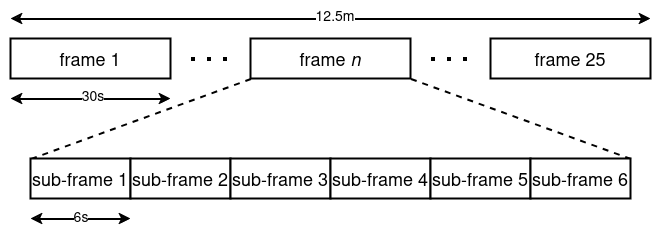
\includegraphics[width=0.75\textwidth]{img/gps_frame}
\end{figure}
\begin{itemize}[nosep]
    \item \textbf{25 frames} (or \textbf{pages}) that takes 12.5 minutes to be transmitted.
    \item each frame takes 30 seconds to be transmitted and it is formed by \textbf{6 sub-frame}.
    \begin{enumerate}[nosep]
        \item the first sub-frame contains the \textbf{satellite clock information}.
        \item the second and the third give the information about the \textbf{satellite ephemeris} (\textbf{orbit}).
        \item the forth and thr fifth are different and are complete only receiving all the 25 frames of the NAV msg, they have the \textbf{Almanac \& constellation status}.
    \end{enumerate}
    \item each sub-frame needs 6 seconds to be transmitted, and it is composed by \textbf{10 words}.
    \item each word consist of \textbf{30 bits} and it takes 0.6 second to be transmitted.
\end{itemize}

\newpage
\subsection{Bit Coding}
GPS use the \textbf{Bi-Phase Shift Key} (\textbf{BPSK}) modulation technique. In BPSK the carrier signal is modified by altering its phase by 180 degree, for each symbol. A phase shift of 180 degrees denotes a binary 0 while no phase shift represents a binary 1. The advantages to use this type of mudaltion technique is:
\begin{enumerate}[nosep]
    \item rendundancy
    \item jamming resistance
    \item measure \& remove the ionospheric delay
    \item requires a dual frequency receiver (with a single one it is possible to survive but less accuracy) one at $1575.42MHz$ and the other one at $1227.60MHz$.
\end{enumerate}
\begin{figure}[h]
    \centering
    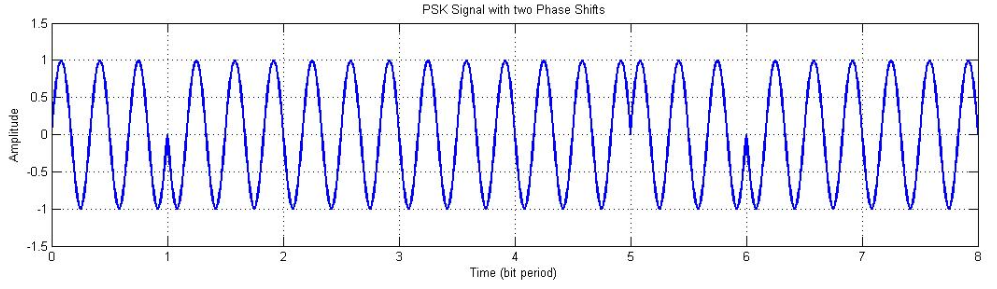
\includegraphics[width=\textwidth]{img/bspk_wave}
\end{figure}
\begin{figure}[h]
    \centering
    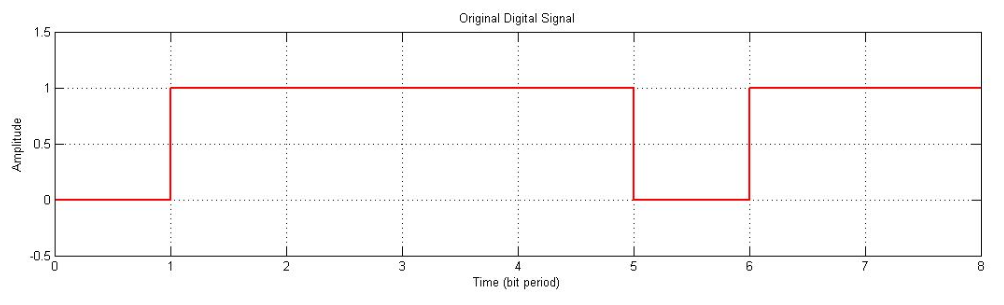
\includegraphics[width=\textwidth]{img/bspk_signal}
\end{figure}

\newpage
\subsection{Working Principle}
Let's distinguish the study of the working principle in two hypotheses: \textbf{theoretical}: receiver clock is perfectly synchronize with the satellite clock (\textit{absolute clock}); and \textbf{reality}: receiver clock is cheap, non-atomic and not perfectly synchronize with the satellite clock.

\begin{figure}[h]
    \centering 
    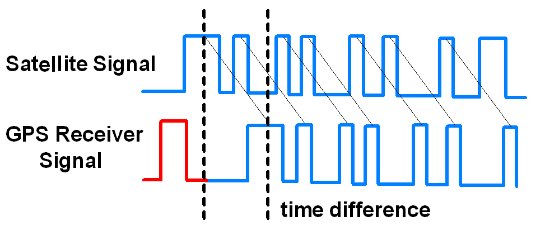
\includegraphics[width=0.45\textwidth]{img/hp_theory}
    \caption{Satellite-Recevier clock synch}
\end{figure}
In the first hypothesis, we know: \textbf{satellite position} (written in the NAV), \textbf{satellite clock} (written in the NAV) and the \textbf{speed of light} $c$. So it is possible to obtain:
\begin{enumerate}[nosep]
    \item \textbf{signal travel time}: $\Delta t = clock_{recv} - clock_{NAV}$
    \item \textbf{distance satellite-receiver}: $d = c \cdot \Delta t$
\end{enumerate}
The problem is, if there is at least $1ms$ of de-sync between the satellite and the receiver, then will have at least an error of 200 miles.
Solution: \textbf{\textit{Trilateration}}.

\begin{figure}[h]
    \centering
    \begin{minipage}[t]{0.3\textwidth}
        \centering
        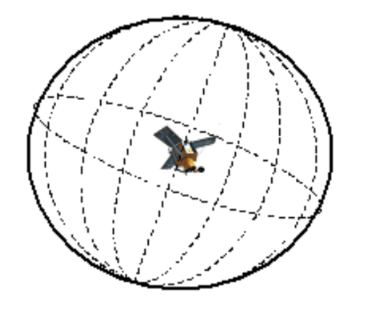
\includegraphics[width=0.7\textwidth]{img/gps_one}

        \begin{flushleft}
            if it is knows \textbf{one} $sat_i$ and the distance $d_i$ we can be in any point of the spherical surface of radius $d_i$ centered in $sat_i$.
        \end{flushleft}
    \end{minipage}
    \begin{minipage}[t]{0.3\textwidth}
        \centering
        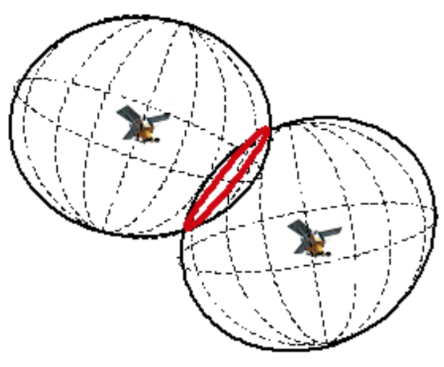
\includegraphics[width=0.7\textwidth]{img/gps_two}

        \begin{flushleft}
            if the sat known are \textbf{two} $sat_i$ and $sat_j$ both the position and the distance $d_i$, $d_j$ we can be in any point of the border given by the intersection of the two sphere's surface.
        \end{flushleft}
    \end{minipage}
    \begin{minipage}[t]{0.3\textwidth}
        \centering
        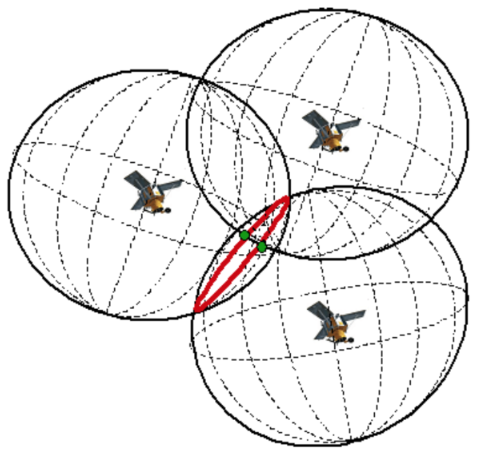
\includegraphics[width=0.7\textwidth]{img/gps_three}

        \begin{flushleft}
            adding the \textbf{third} sat, we have \textbf{three} sphere, that ends the intersection with two available points. One is on the Earth surface (us) the other is in the open space (discard).
        \end{flushleft}
    \end{minipage}
\end{figure}
In the \textbf{reality} the satellite and the receiver do not have the clock synchronize, so it is important to introduce a factor named \textit{clock error} $\Delta e$:
\begin{center}
    $d_i = \sqrt{(x_i - x_u)^2 + (y_i - y_u)^2 + (z_i - z_u)^2} + c \cdot \Delta e$
\end{center}
where:
\begin{itemize}[nosep]
    \item $x_i$, $y_i$ and $z_i$ are the sat position, \textbf{know} (NAV).
    \item $c$ is the speed of light, \textbf{know}.
    \item $x_u$, $y_u$ and $z_u$ are the position of the receiver, \textbf{unknown}.
    \item $\Delta e$ is the clock error, \textbf{unknown}.
\end{itemize}
If we consider four satellites $sat_i$, $sat_j$, $sat_k$ and $sat_p$ we end with four equations and four unknown items: $x_u$, $y_u$, $z_u$ and $\Delta e$.
\begin{center}
    \begin{math}
        \begin{cases}
            d_i = \sqrt{(x_i - x_u)^2 + (y_i - y_u)^2 + (z_i - z_u)^2} + c \cdot \Delta e \\
            d_j = \sqrt{(x_j - x_u)^2 + (y_j - y_u)^2 + (z_j - z_u)^2} + c \cdot \Delta e \\
            d_k = \sqrt{(x_k - x_u)^2 + (y_k - y_u)^2 + (z_k - z_u)^2} + c \cdot \Delta e \\
            d_p = \sqrt{(x_p - x_u)^2 + (y_p - y_u)^2 + (z_p - z_u)^2} + c \cdot \Delta e
        \end{cases}
    \end{math}
\end{center}
$\Delta e$ is equal for all satellite, because all of them are perfectly synchronize, so the \textit{clock error} is the same for each tuples (sat, recv). If recv and sat are perfectly synchronize (\textbf{time} given), with just 3 sat is possible to calculate your position. If you know where you are (\textbf{space} given), with just one sat is possible to have the clock sync, but if you do \textbf{not know} both \textbf{space} and \textbf{time} you need at least four sat to solve the equation.

\subsection{GPS limitation}
\begin{itemize}[nosep]
    \item it require a lot of power to work properly.
    \item GPS signal do not pass solid structure.
    \item affected by large buildings, unreliable in dense urban area.
    \item GPS accuracy is function of the signal reception, larger the antenna, better the signal. $miniaturization \quad \frac{1}{\alpha} \quad accuracy$
\end{itemize}

\newpage
\section{Bluetooth}
\textbf{\textit{Bluetooth}} is short-range wireless technology and it was introduce for the first time in 1994 to replace serial \textit{RS-232} wired cables. Typically used for \textbf{point-to-point} technologies. It has a coverage of 10m and creates a network named \textbf{Personal Area Network} (\textbf{PAN}), the frequency range is between $2.4GHz$ and $2.485GHz$ with few $Mbps$ of bandwidth. It is standardize in the \textit{IEEE 802.15.1} like packet-base protocol.

\begin{figure}[h]
    \centering
    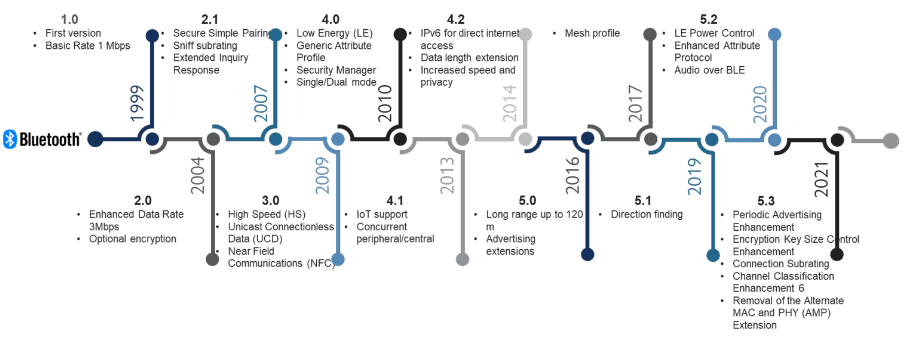
\includegraphics[width=\textwidth]{img/bluetooth_timeline}
    \caption{Bluetooth different version in the time}
\end{figure}
